\section{Estructura y codificación de las máquinas de estado}

Como se anticipó al describir la arquitectura, la recepción, la transmisión y el
control de cada operación avanzan por etapas y necesitan conservar su progreso
entre ciclos de reloj. Por ese motivo se utilizaron tres máquinas de estado: RX,
TX y el controlador.

Las tres FSM comparten la misma estructura: un registro de estado, lógica
combinacional para determinar el próximo estado y las salidas, constantes
locales para representar cada etapa y una rama \texttt{default} que permite
regresar a IDLE ante una codificación no contemplada.

Se eligió la codificación one-hot para las tres FSM. En este tipo de
codificación cada estado ocupa un flip-flop y solo un bit debe
permanecer activo. Esta representación consume más registros que una
codificación binaria, pero simplifica la lógica de decodificación en
FPGA y hace visibles los estados durante la depuración. RX utiliza
cinco bits, TX cuatro y el controlador cinco. El atributo
\texttt{fsm\_encoding = one\_hot} conserva esta intención durante la
extracción y optimización de las máquinas en Vivado.

En una codificación binaria cinco estados requerirían tres bits y
cada transición debería decodificar una combinación. En la
codificación one-hot se reservan cinco bits, por ejemplo
\texttt{00001} para IDLE y \texttt{00100} para DATA. El costo
adicional es de dos flip-flops; la ventaja es que comprobar ``estoy
en DATA'' se reduce conceptualmente a observar un solo bit. Esto no
elimina la necesidad de describir qué ocurre ante \texttt{00000} o
ante dos bits activos: la rama \texttt{default} devuelve la FSM al estado IDLE.

\begin{codebox}[language=SystemVerilog]
	(* fsm_encoding = "one_hot" *) reg [4:0] state = STATE_IDLE;
	reg [4:0] next_state;

	always @(posedge clk) begin
	if (reset) state <= STATE_IDLE;
	else       state <= next_state;
	end

	always_comb begin
	next_state = state;
	case (state)
	// cada estado modifica solo las senales necesarias
	default: next_state = STATE_IDLE;
	endcase
	end
\end{codebox}

El registro secuencial \texttt{state} representa el estado actual. El
bloque combinacional calcula el próximo estado \texttt{next\_state} y
las salidas a partir de entradas y registros.

\section{Receptor UART}

La FSM del receptor separa reposo, validación del bit de start,
recepción de los datos, validación del bit de stop y recuperación.
Sus transiciones principales se resumen en la figura~\ref{fig:fsm-rx}.

\begin{figure}[H]
	\centering
	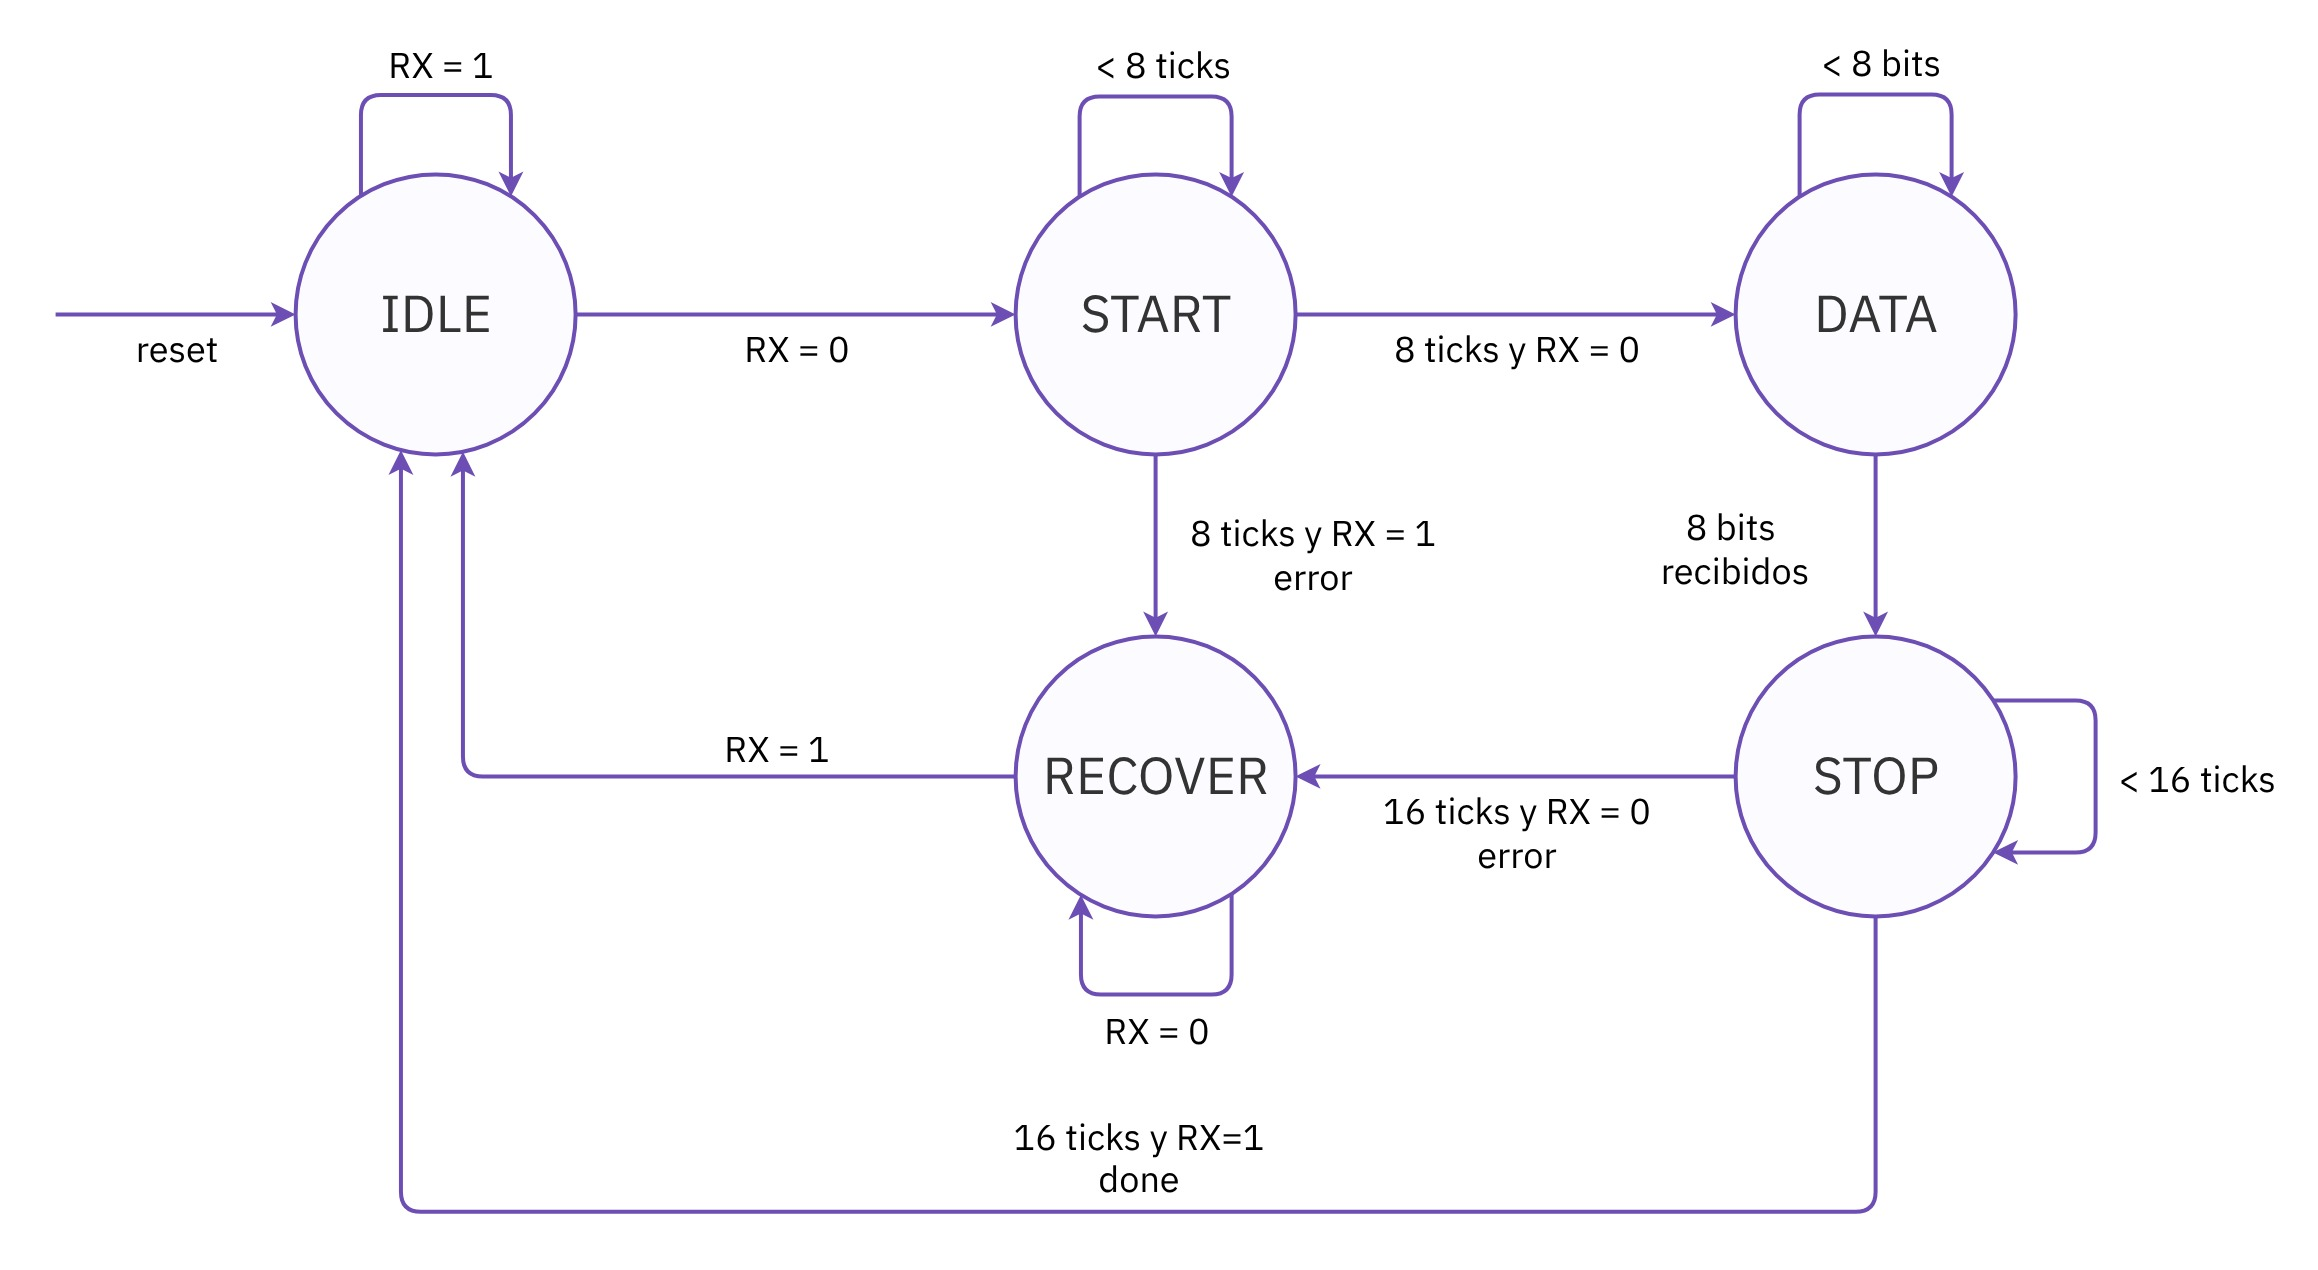
\includegraphics[width=0.94\textwidth]{img/fsm_rx.jpg}
	\caption{Estados y condiciones principales del receptor.}%
	\label{fig:fsm-rx}
\end{figure}

\subsection{Validación del bit de start}

En IDLE, una entrada baja inicia la observación. La FSM no la acepta
de inmediato si no que espera ocho ticks, es decir, medio período de
bit para sobremuestreo 16x. Si RX continúa bajo, el punto observado
corresponde al centro del start y se pasa a DATA. Si volvió a alto,
se trata de un pulso espurio por lo que se genera un único
\texttt{frame\_error\_tick} y se ingresa en RECOVER.

\subsection{Muestreo y orden de bits}

Después del centro del start, cada dato se toma al completar
dieciséis ticks. Como UART envía D0 primero, la nueva muestra entra
por el bit más significativo de un registro que se desplaza a la derecha:

\begin{codebox}[language=SystemVerilog]
	next_data = {rx, data_reg[DATA_BITS-1:1]};
\end{codebox}

Tras ocho iteraciones, las muestras quedan en su posición natural. Se
espera entonces un período completo de stop. Solo si RX es alto se
genera \texttt{rx\_done\_tick}; un stop bajo no publica el byte.

\subsection{Estado de recuperación}

Después de un falso start o de un stop inválido, la línea puede
permanecer baja durante varios bits. Si se volviera inmediatamente a
IDLE se generaría un error repetido por cada nueva observación de ese
mismo nivel. RECOVER mantiene los contadores en cero y espera el
retorno a reposo en alto antes de habilitar otra trama. Así, cada
evento defectuoso produce un solo pulso de error.

\section{Transmisor UART}

El transmisor recibe un byte completo, pero debe enviarlo por
\texttt{tx} un bit a la vez y respetar la duración de cada parte de la trama
8N1. Una máquina de estados conserva el avance de esa secuencia. Como todos los
niveles de salida son generados por el propio circuito, se requieren cuatro
estados: IDLE, START, DATA y STOP.

En IDLE, la línea permanece en alto. Un pulso en \texttt{tx\_start} hace que el
módulo guarde \texttt{data\_in} y comience el bit de start en nivel bajo. Luego
transmite los ocho bits de datos desde D0 hasta D7 y finaliza con el bit de stop
en alto. Cada bit se mantiene durante dieciséis pulsos de \texttt{s\_tick}.

\begin{figure}[H]
	\centering
	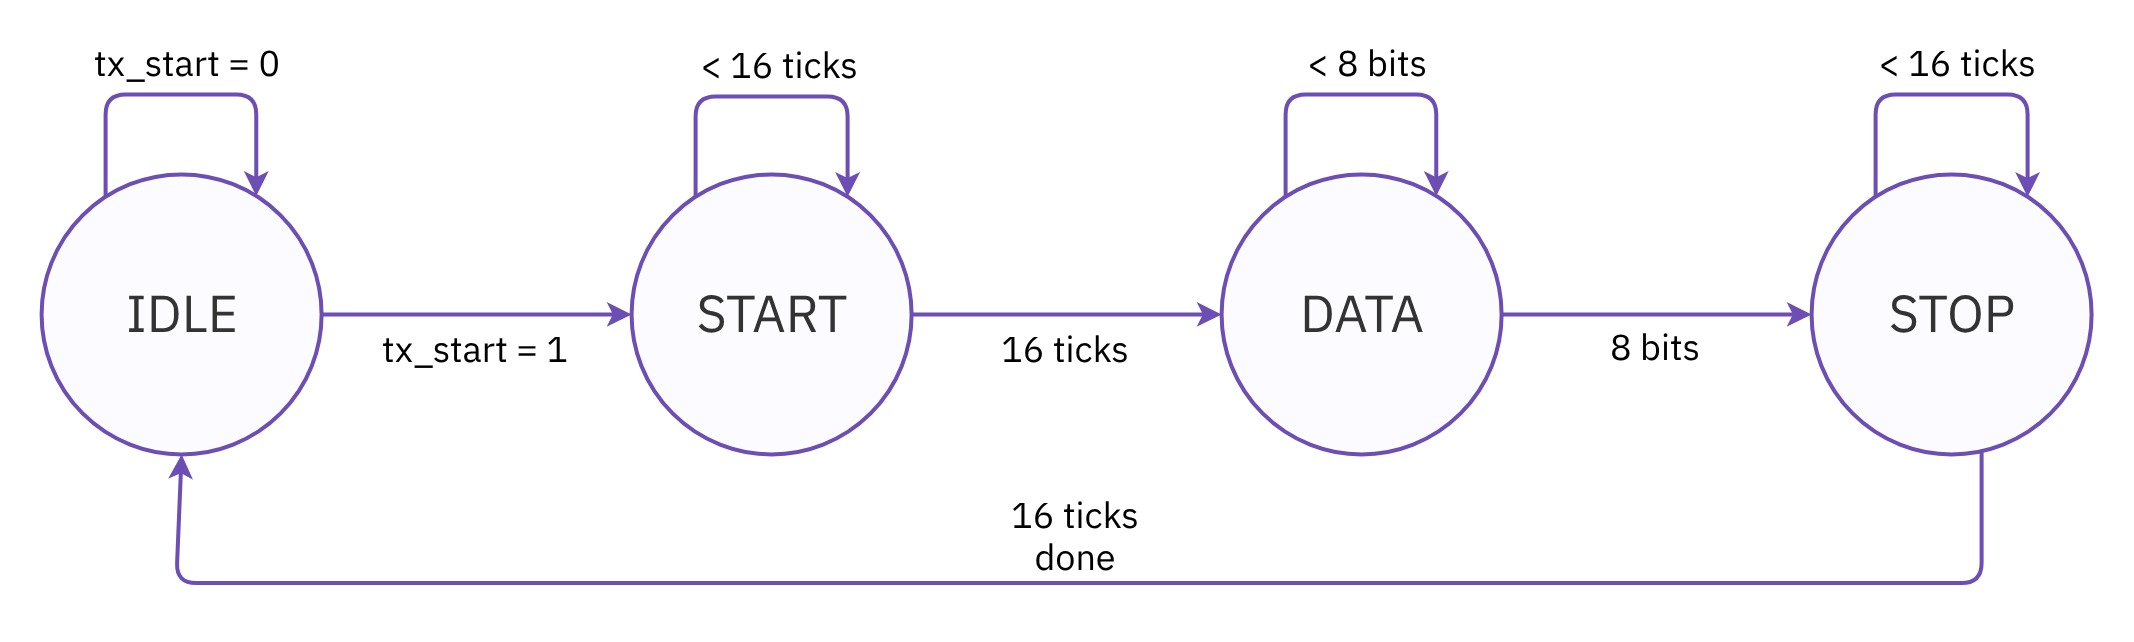
\includegraphics[width=0.86\textwidth]{img/fsm_tx.jpg}
	\caption{Secuencia de estados del transmisor.}%
\end{figure}

Mientras la trama está en curso, \texttt{tx\_busy} permanece activo. Al
completar el stop, \texttt{tx\_done\_tick} se activa durante un ciclo y permite
que el núcleo retire el byte del FIFO. Si todavía quedan datos pendientes, una
nueva activación de \texttt{tx\_start} inicia la trama siguiente.

El byte se copia a un registro interno al comenzar la transmisión. Así conserva
el mismo valor durante toda la trama, aunque \texttt{data\_in} cambie antes de
que finalice. Al terminar cada período de bit, el registro se desplaza para
presentar el dato siguiente:

\begin{codebox}[language=SystemVerilog]
	if (tx_start) begin
	next_state = STATE_START;
	next_data  = data_in;
	next_tx    = 1'b0;
	end
	// ... al terminar cada dato
	next_data = {1'b0, data_reg[DATA_BITS-1:1]};
	next_tx   = data_reg[1];
\end{codebox}

\section{Buffers FIFO}

La UART y el controlador no siempre están listos en el mismo ciclo. El FIFO se
ubica entre ambos y conserva temporalmente los bytes, de modo que el productor
puede escribir sin esperar que el consumidor los retire de inmediato. Una
escritura se acepta mientras exista espacio y una lectura, mientras haya datos
disponibles.

Cada FIFO puede almacenar cuatro bytes. El registro
\texttt{read\_pointer} señala el byte que se leerá a continuación,
mientras que \texttt{write\_pointer} indica la posición de la próxima
escritura. Ambos avanzan de forma circular: después de la última
posición regresan a la primera.

El registro \texttt{count} indica cuántos bytes contiene la cola.
Este valor permite distinguir entre vacío y lleno incluso cuando los
dos punteros coinciden. Si una lectura y una escritura se aceptan en
el mismo ciclo, sale un byte y entra otro, por lo que la cantidad de
datos almacenados no cambia.

\begin{codebox}[language=SystemVerilog]
	assign empty = (count == 0);
	assign full  = (count == DEPTH);
	assign read_accept  = rd && !empty;
	assign write_accept = wr && !full;

	case ({write_accept, read_accept})
	2'b10:   count <= count + 1'b1;
	2'b01:   count <= count - 1'b1;
	default: count <= count;
	endcase
\end{codebox}

Si la cola está llena al comenzar el ciclo, no puede aceptar una
nueva escritura, aunque \texttt{rd} y \texttt{wr} se activen al mismo
tiempo. En ese flanco se realiza solamente la lectura, que libera una
posición. La escritura puede repetirse en el ciclo siguiente, cuando
ya existe espacio disponible. De esta forma se evita sobrescribir el
dato más antiguo. Este caso también se comprueba en \texttt{fifo\_tb}.

\section{Controlador de transacciones}

La tercera FSM traduce bytes completos al contrato de la ALU. En el
estado WAIT\_A consume el primer elemento de la cola de recepción y
carga el operando A. En los estados WAIT\_B y WAIT\_OPCODE se hace lo
mismo para el operando B y el opcode. El estado de EXECUTE reserva un
ciclo para registrar el resultado y mostrar los indicadores. El
estado de WAIT\_TX conserva esos registros si la cola de transmisión
está llena y escribe cuando existe espacio en la misma.

\begin{figure}[H]
	\centering
	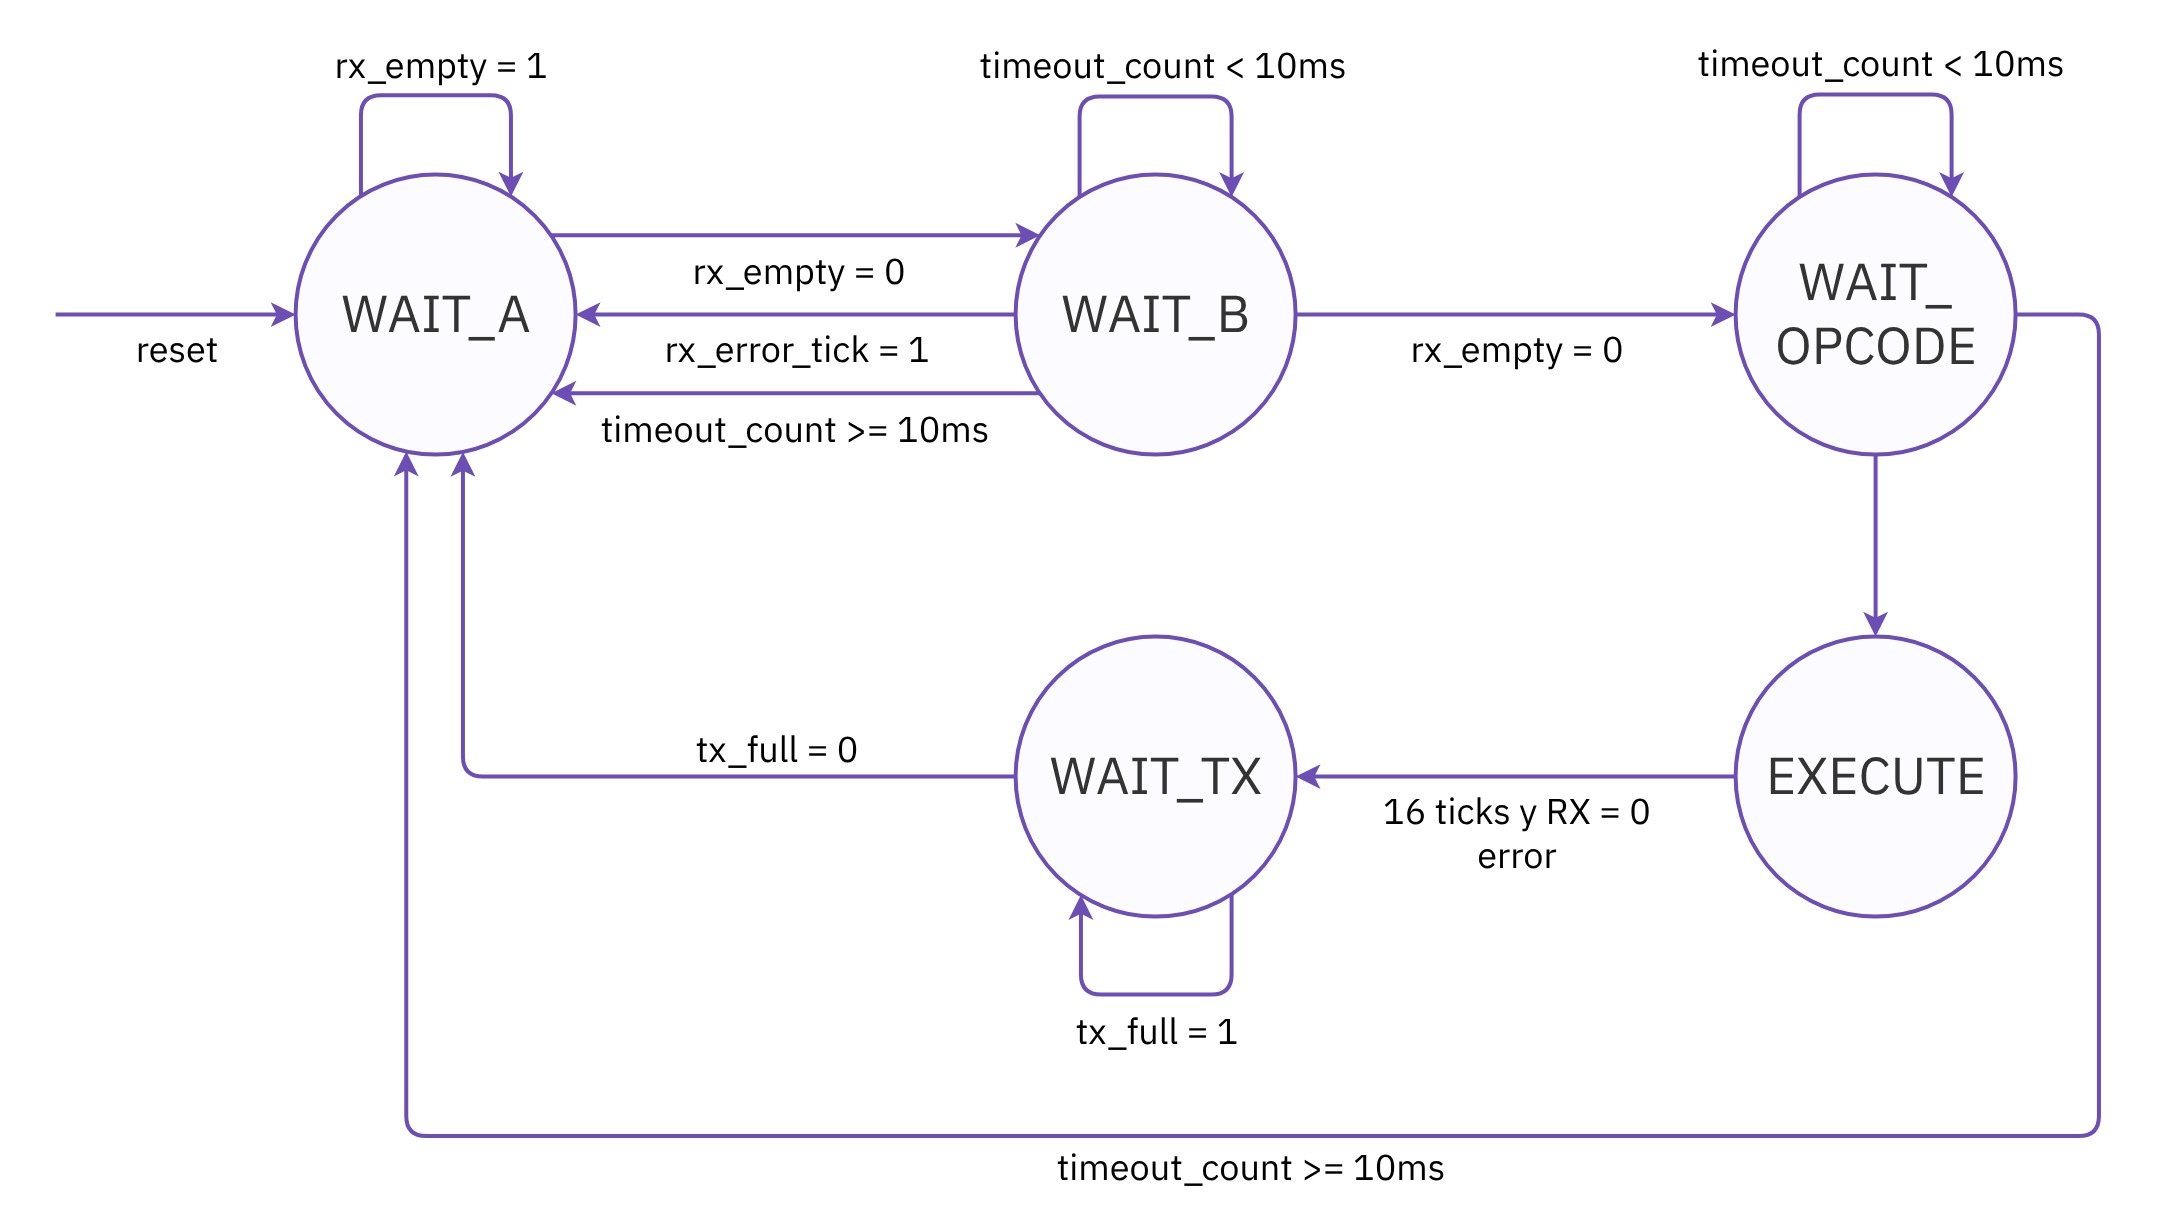
\includegraphics[width=0.875\textwidth]{img/fsm_controller.jpg}
	\caption{FSM que delimita una operación de tres bytes.}%
\end{figure}

El timeout solo es necesario después de recibir el primer operando y antes de
completar la solicitud. Por eso el contador avanza mientras el controlador
espera B o el opcode, y vuelve a cero cada vez que llega un byte
válido. Mientras
se espera A permanece inactivo. Si vence el plazo o RX informa un error durante
una solicitud parcial, los datos recibidos se descartan y el controlador vuelve
a WAIT\_A.

Cuando llega el opcode, su registro se actualiza al finalizar el
flanco de reloj.
El resultado de la ALU no puede capturarse en ese mismo instante porque todavía
depende del valor anterior. El estado EXECUTE proporciona un ciclo adicional
para que A, B y opcode permanezcan estables y la ALU produzca el resultado
correcto. Después, WAIT\_TX conserva ese resultado y sus banderas hasta que haya
espacio en la cola de transmisión.

\begin{codebox}[language=SystemVerilog]
	STATE_EXECUTE: begin
	capture_result = 1'b1;
	next_state = STATE_WAIT_TX;
	end

	STATE_WAIT_TX: begin
	if (!tx_full) begin
	wr_uart = 1'b1;
	next_state = STATE_WAIT_A;
	end
	end
\end{codebox}

\section{Recuperación de estados ilegales}

En una codificación one-hot, solo son válidas las combinaciones que tienen un
único bit activo. Una perturbación podría modificar el registro y producir una
combinación que no represente ningún estado definido. Para evitar que la máquina
quede detenida en esa situación, cada sentencia \texttt{case} incluye una rama
\texttt{default}.

Ante un estado no reconocido, las FSM de RX y TX regresan a IDLE y restablecen
sus registros auxiliares. El controlador vuelve a WAIT\_A para comenzar una
solicitud nueva. De este modo, todas las combinaciones posibles conducen a un
comportamiento definido y la operación puede continuar desde un estado conocido
en el ciclo siguiente.
